\section{\textit{Karolina Rozmus}}
\label{sec:krozmus}

Do you see this cat? He is saying "hi" to you! (see Figure~\ref{fig:animals}).
\begin{figure}[H]
    \centering
    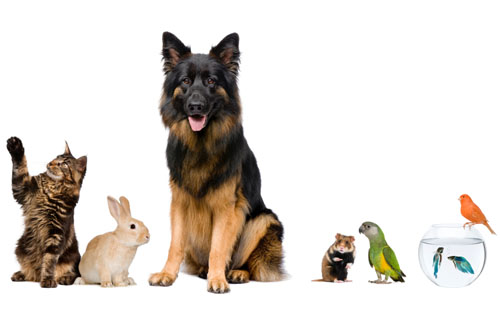
\includegraphics[width=0.8\textwidth]{pictures/pic_Krozmus.jpg} 
    \caption{This picture shows the most popular animals kept in polish households.}
    \label{fig:animals}
\end{figure}


Table~\ref{tab:animals} shows how many people (in percent) has a specific animal. 

\begin{table}[H]
    \centering
    \begin{table}[htbp]
\centering
\begin{tabular}{||c c c c c||} 
 \hline
 Country & Dog & Hamster & Fish & Cat \\ [0.5ex] 
 \hline\hline
 Poland & 47\% & 13\% & 21\% & 60\% \\ 
 \hline
 Germany & 52\% & 8\% & 30\% & 45\% \\
 \hline
 England & 56\% & 30\% & 7\% & 29\% \\
 \hline
 United States & 61\% & 9\% & 15\% & 61\% \\
 \hline
 Italy & 29\% & 3\% & 8\% & 44\% \\
 \hline
\end{tabular}
\label{tab:animals}
\caption{Please do not check the authenticity of the data.}
\end{table}
\end{table}


Here you can see the most popular mathematical formula in the world. \[a^2 + b^2 = c^2\]




\textbf{Something about C:\\}

C is a general-purpose programming language created by Dennis Ritchie at the Bell Laboratories in 1972.

It is a very popular language, despite being old. The main reason for its popularity is because it is a fundamental language in the field of computer science.

C is strongly associated with UNIX, as it was developed to write the UNIX operating system.
\\

\textbf{This is the list of the best Barbie movies:}

\begin{itemize}
  \item 'Barbie and the Three Musketeers' (2009)
  \item 'Barbie Fairytopia: Mermaidia' (2006)
  \item 'Barbie as the Island Princess' (2007)
  \item 'Barbie and the Diamond Castle' (2008)
  \item 'Barbie: Fairytopia' (2005)
  \end{itemize}

\textbf{And this is the rest of the list, but with numbers:}

\begin{enumerate}
  \item 'Barbie of Swan Lake' (2003)
  \item 'Barbie in the 12 Dancing Princesses' (2006)
  \item 'Barbie as Rapunzel' (2002)
  \item 'Barbie as the Princess and the Pauper' (2004)
  \item 'Barbie in the Nutcracker' (2001)
\end{enumerate}









